\subsection{bpmdsp/bpm\_\-dsp.h File Reference}
\label{bpm__dsp_8h}\index{bpmdsp/bpm\_\-dsp.h@{bpmdsp/bpm\_\-dsp.h}}


\subsubsection{Detailed Description}
libbpm digital signal processing routines 



Definition in file {\bf bpm\_\-dsp.h}.

{\tt \#include $<$stdio.h$>$}\par
{\tt \#include $<$stdlib.h$>$}\par
{\tt \#include $<$string.h$>$}\par
{\tt \#include $<$math.h$>$}\par
{\tt \#include \char`\"{}bpm/bpm\_\-defs.h\char`\"{}}\par
{\tt \#include \char`\"{}bpm/bpm\_\-messages.h\char`\"{}}\par
{\tt \#include \char`\"{}bpm/bpm\_\-nr.h\char`\"{}}\par
{\tt \#include \char`\"{}bpm/bpm\_\-wf.h\char`\"{}}\par


Include dependency graph for bpm\_\-dsp.h:\nopagebreak
\begin{figure}[H]
\begin{center}
\leavevmode
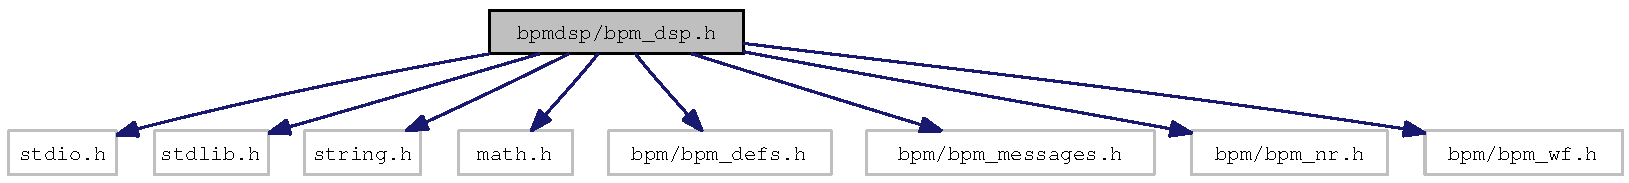
\includegraphics[width=409pt]{bpm__dsp_8h__incl}
\end{center}
\end{figure}


This graph shows which files directly or indirectly include this file:\nopagebreak
\begin{figure}[H]
\begin{center}
\leavevmode
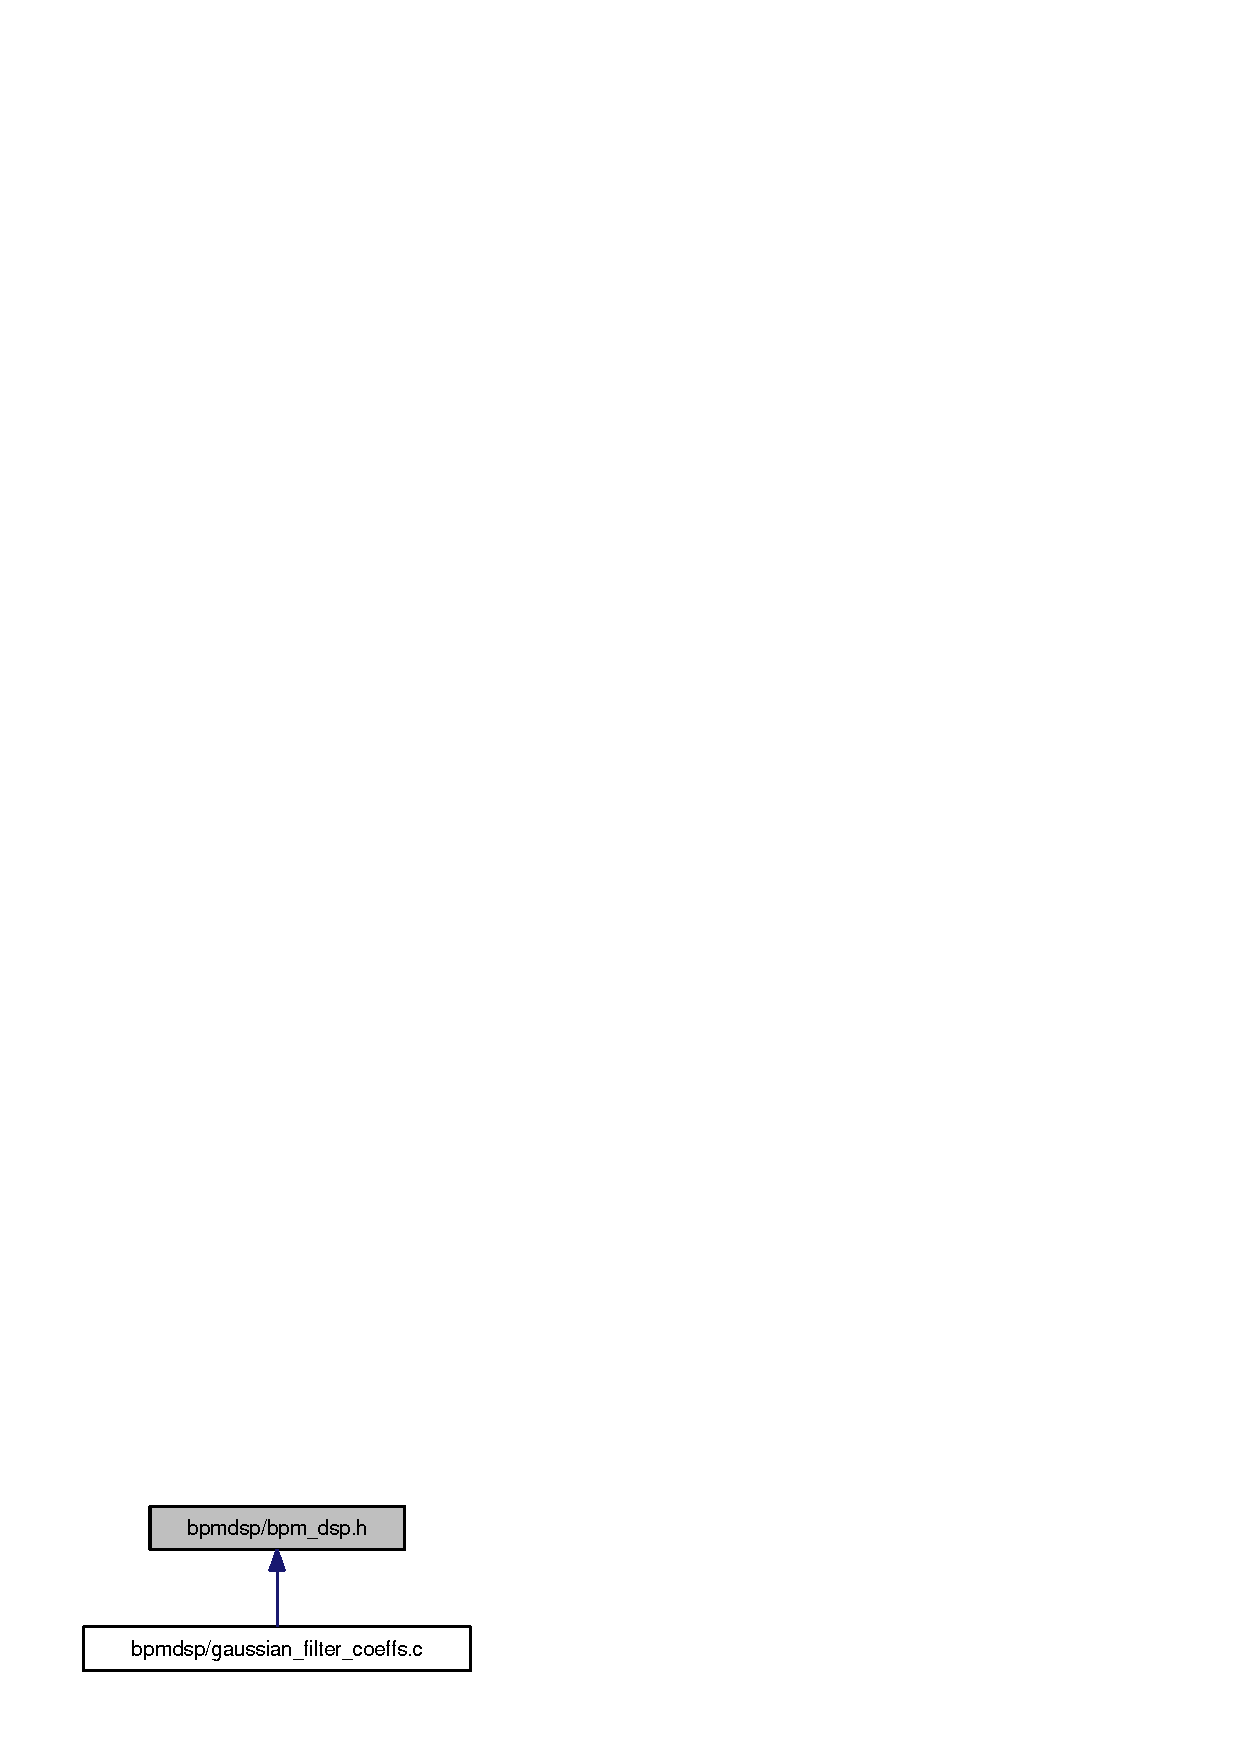
\includegraphics[width=115pt]{bpm__dsp_8h__dep__incl}
\end{center}
\end{figure}
\subsubsection*{Data Structures}
\begin{CompactItemize}
\item 
struct {\bf filterrep\_\-t}
\item 
struct {\bf filter\_\-t}
\end{CompactItemize}
\subsubsection*{Defines}
\begin{CompactItemize}
\item 
\#define {\bf BESSEL}
\item 
\#define {\bf BUTTERWORTH}
\item 
\#define {\bf CHEBYSHEV}
\item 
\#define {\bf RAISEDCOSINE}
\item 
\#define {\bf RESONATOR}
\item 
\#define {\bf GAUSSIAN}
\item 
\#define {\bf BILINEAR\_\-Z\_\-TRANSFORM}
\item 
\#define {\bf MATCHED\_\-Z\_\-TRANSFORM}
\item 
\#define {\bf NO\_\-PREWARP}
\item 
\#define {\bf CAUSAL}
\item 
\#define {\bf ANTICAUSAL}
\item 
\#define {\bf NONCAUSAL}
\item 
\#define {\bf GAUSSIAN\_\-SIGMA\_\-BW}
\item 
\#define {\bf LOWPASS}
\item 
\#define {\bf HIGHPASS}
\item 
\#define {\bf BANDPASS}
\item 
\#define {\bf BANDSTOP}
\item 
\#define {\bf NOTCH}
\item 
\#define {\bf ALLPASS}
\item 
\#define {\bf FIR}
\item 
\#define {\bf IIR}
\item 
\#define {\bf MAXORDER}
\item 
\#define {\bf MAXPZ}
\item 
\#define {\bf FILT\_\-EPS}
\item 
\#define {\bf MAX\_\-RESONATOR\_\-ITER}
\item 
\#define {\bf FFT\_\-FORWARD}
\item 
\#define {\bf FFT\_\-BACKWARD}
\end{CompactItemize}
\subsubsection*{Functions}
\begin{CompactItemize}
\item 
EXTERN {\bf filter\_\-t} $\ast$ {\bf create\_\-filter} (char name[$\,$], unsigned int options, int order, int ns, double fs, double f1, double f2, double par)
\item 
EXTERN int {\bf apply\_\-filter} ({\bf filter\_\-t} $\ast$f, {\bf doublewf\_\-t} $\ast$w)
\item 
EXTERN void {\bf print\_\-filter} (FILE $\ast$of, {\bf filter\_\-t} $\ast$f)
\item 
EXTERN void {\bf delete\_\-filter} ({\bf filter\_\-t} $\ast$f)
\item 
EXTERN int {\bf filter\_\-step\_\-response} ({\bf filter\_\-t} $\ast$f, {\bf doublewf\_\-t} $\ast$w, int itrig)
\item 
EXTERN int {\bf filter\_\-impulse\_\-response} ({\bf filter\_\-t} $\ast$f, {\bf doublewf\_\-t} $\ast$w, int itrig)
\item 
EXTERN {\bf filterrep\_\-t} $\ast$ {\bf create\_\-splane\_\-representation} ({\bf filter\_\-t} $\ast$f)
\item 
EXTERN {\bf filterrep\_\-t} $\ast$ {\bf create\_\-resonator\_\-representation} ({\bf filter\_\-t} $\ast$f)
\item 
EXTERN {\bf filterrep\_\-t} $\ast$ {\bf zplane\_\-transform} ({\bf filter\_\-t} $\ast$f, {\bf filterrep\_\-t} $\ast$s)
\item 
EXTERN void {\bf print\_\-filter\_\-representation} (FILE $\ast$of, {\bf filterrep\_\-t} $\ast$r)
\item 
EXTERN int {\bf normalise\_\-filter} ({\bf filter\_\-t} $\ast$f, {\bf filterrep\_\-t} $\ast$s)
\item 
EXTERN int {\bf calculate\_\-filter\_\-coefficients} ({\bf filter\_\-t} $\ast$f)
\item 
EXTERN int {\bf gaussian\_\-filter\_\-coeffs} ({\bf filter\_\-t} $\ast$f)
\item 
EXTERN int {\bf \_\-expand\_\-complex\_\-polynomial} ({\bf complex\_\-t} $\ast$w, int n, {\bf complex\_\-t} $\ast$a)
\item 
EXTERN {\bf complex\_\-t} {\bf \_\-eval\_\-complex\_\-polynomial} ({\bf complex\_\-t} $\ast$a, int n, {\bf complex\_\-t} z)
\item 
EXTERN int {\bf ddc\_\-initialise} (int ns, double fs)
\item 
EXTERN void {\bf ddc\_\-cleanup} (void)
\item 
int {\bf ddc} ({\bf doublewf\_\-t} $\ast$w, double f, {\bf filter\_\-t} $\ast$filter, {\bf complexwf\_\-t} $\ast$dcw, {\bf doublewf\_\-t} $\ast$bufre, {\bf doublewf\_\-t} $\ast$bufim)
\item 
EXTERN int {\bf fft\_\-gen\_\-tables} (void)
\item 
EXTERN int {\bf fft\_\-initialise} (int ns)
\item 
EXTERN void {\bf fft\_\-cleanup} (void)
\item 
EXTERN int {\bf complexfft} ({\bf complexwf\_\-t} $\ast$z, int fft\_\-mode)
\item 
EXTERN int {\bf realfft} ({\bf doublewf\_\-t} $\ast$y, int fft\_\-mode, {\bf complexwf\_\-t} $\ast$z)
\item 
EXTERN void {\bf norm\_\-phase} (double $\ast$phase)
\end{CompactItemize}
